\chapter{Introduction}


 \fei{What is the problem here?  Why is it hard?}
 \fei{IMportant: use a picture and a motivating example to demonstrate and show the above points in a realistic setting.  This will help reader understand the problem, how it occurs in real life and why it's hard.}
\fei{Briefly describe 2-3 related work techniques (high level) and state why they are not sufficient, state technical weaknesses.  I suggest you focus on NormA, SAND, DAMP.}


\section{Problem Domain and Motivation}

A time series is a sequence of observations recorded over time. Time-series data are common in many real-world applications, such as electrocardiogram (ECG) monitoring, electricity demand forecasting, and financial markets \citep{schmidl2022anomaly}. Unlike ordinary data, the order of observations in a time series is important. The meaning of a value depends not only on its magnitude, but also on when it occurs and how it relates to surrounding observations.

The goal of time-series anomaly detection is to find unusual patterns in a time series \citep{chandola2009anomaly}. Anomalies can occur at different temporal scales. An anomaly may appear as a single observation, such as an isolated spike in a sensor reading. The anomaly may also span a short interval whose overall shape differs from the rest of the time series, even though no individual observation is particularly extreme. Contextual anomalies depend on the surrounding circumstances and may be considered abnormal only under specific conditions, such as an elevated heart rate during rest but not during exercise. Detecting these anomalies requires considering observed values and the context in which they occur.

Concept drift refers to a change in the underlying data distribution over time \citep{gama2014survey,lu2019learning}. In time-series anomaly detection, the definition of normal behavior maybe not be fixed. For example, electricity usage may change between weekdays and weekends, weather measurements may shift gradually across seasons, and ECG patterns may change when a patient's activity or physiological condition changes. A changed pattern may be either a true anomaly or an actual new normal state.

For example, in Figure Figure~\ref{fig11}, the first region represents an old normal pattern. Later, the data gradually changes into a new normal pattern. A detector that compares all future points against only the old normal pattern may incorrectly flag the drift and new normal region as anomalous. However, a detector that adapts without control may also miss the true anomaly. This is the main challenge addressed in this report: anomalies and drift can look similar in the signal, but they require different interpretations.

\begin{figure}[H]
\centering
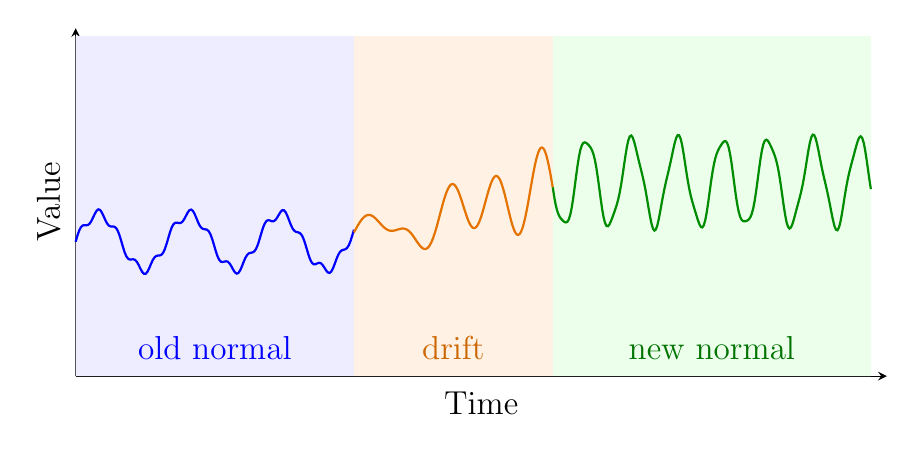
\begin{tikzpicture}
\begin{axis}[
    width=0.98\textwidth,
    height=6.0cm,
    xlabel={Time},
    ylabel={Value},
    xmin=0, xmax=102,
    ymin=-1.7, ymax=2.7,
    axis lines=left,
    xtick=\empty,
    ytick=\empty,
    clip=false,
    label style={font=\large},
    tick label style={font=\small}
]

\addplot[draw=none, fill=blue!7] coordinates {(0,-1.7) (35,-1.7) (35,2.6) (0,2.6)} \closedcycle;
\addplot[draw=none, fill=orange!10] coordinates {(35,-1.7) (60,-1.7) (60,2.6) (35,2.6)} \closedcycle;
\addplot[draw=none, fill=green!8] coordinates {(60,-1.7) (100,-1.7) (100,2.6) (60,2.6)} \closedcycle;

\addplot[blue, thick, domain=0:35, samples=160]
{0.35*sin(deg(0.55*x)) + 0.06*sin(deg(2.7*x))};

\addplot[orange!90!black, thick, domain=35:60, samples=220]
{0.30*sin(deg(0.55*x))*(1-(x-35)/25) + 0.55*sin(deg(1.1*x))*((x-35)/25) + 0.028*(x-35)};

\addplot[green!55!black, thick, domain=60:100, samples=220]
{0.55*sin(deg(1.1*x)) + 0.75 + 0.06*sin(deg(3*x))};
\node[blue, font=\large] at (axis cs:17.5,-1.35) {old normal};
\node[orange!80!black, font=\large] at (axis cs:47.5,-1.35) {drift};
\node[green!45!black, font=\large] at (axis cs:80,-1.35) {new normal};

\end{axis}
\end{tikzpicture}
\caption{Illustration of anomaly detection under concept drift.}
\label{fig11}
\end{figure}

Existing time-series anomaly detection methods provide important foundations for this problem. A common workflow in these methods is to first assign an anomaly score to each point, and then convert these scores into binary anomaly labels using a threshold. NormA learns a normal model from representative subsequences and scores new subsequences according to their distance from this model \citep{boniol2021norma}. SAND extends subsequence anomaly detection to streaming data and updates its model as new observations arrive \citep{boniol2021sand}.DAMP is designed for streaming anomaly detection and uses Matrix Profile techniques to identify subsequences that are highly dissimilar to previously normal patterns \citep{lu2022damp}. The final detection result still depends strongly on threshold selection.

Choosing the threshold is difficult in practice. A global threshold may work for datasets which contain similar normal patterns, but it may fail when the data contain drift. When the normal behavior changes, the anomaly-score distribution may also change. As a result, a strict threshold may incorrectly classify drift-driven normal behavior as anomalous, while a loose threshold may miss true abnormal anomalies.

AnDri algorithm addresses this challenge by considering anomaly detection and concept drift detection together \citep{park2025andri,park2025adaptive}. Andri algorithm does not use a single global threshold. It maintains multiple normal patterns and updates them as the data changed. This allows the system to distinguish anomalies from changes caused by concept drift.

In addition to AnDri's anomaly and drift co-detection framework, the system supports an interactive feedback process for refining detection results. Users can review uncertain candidates selected by the system and indicate whether each candidate is normal or anomalous. The feedback is then used to refine the threshold that converts anomaly scores into final predictions. This workflow supports AnDri and baseline methods in the system. As a result, the system serves not only as an implementation of AnDri, but also as an interactive application for exploring, comparing, and evaluating different time-series anomaly detection methods.

\section{Project Goals}

The goal of this project is to build and explain an interactive system for anomaly and drift co-detection in time-series data. The system should not only compute anomaly scores, but also help the user understand why a region is suspicious and whether it is more likely to be a true anomaly or a drift-driven normal change.

The first goal is to support co-detection of anomalies and drift. Co-exploration means that the user can inspect suspicious regions together with their surrounding time-series context, normal-pattern information, anomaly scores, thresholds, and baseline results.

The second goal is to provide a visual workflow for long time series. The system allows the user to upload or select a dataset, choose training regions, mark anomaly examples, review uncertain candidates, and compare final results. This workflow is important because many time-series datasets contain tens or hundreds of thousands of points, making manual inspection difficult without interactive zooming, selection, and summary views.

The third goal is to enable adaptive threshold adjustment based on user feedback. Most anomaly detection methods, including AnDri and baseline methods such as NormA, SAND, and DAMP, produce anomaly scores before applying a threshold to decide which points or subsequences are anomalous. However, this threshold is difficult to set manually because score distributions vary across datasets, methods, and normal patterns. The system therefore allows the user to review candidate anomalies, provide feedback, and adjust the threshold dynamically. In AnDri, this process supports pattern-aware interpretation under concept drift. For baseline methods, the same feedback process allows users to calibrate fixed-threshold results more carefully instead of accepting a single automatic cutoff.

\section{Contributions}

The normal-pattern learning component used by AnDri, including Adjacent Hierarchical Clustering, belongs to the broader AnDri research work and is treated in this report as prior methodology. It is not my individual contribution. My individual contributions focus on the surrounding system implementation, interaction workflow, visualization, evaluation support, and deployment.

\begin{enumerate}
    \item \textbf{Interactive AnDri demonstration system.} Implemented and integrated a browser-based system that supports the end-to-end workflow for time-series anomaly and drift exploration. The system connects data loading, training-region selection, anomaly labeling, candidate review, algorithm execution, and result comparison in one interface.

    \item \textbf{Visual analytics workflow for anomaly and drift co-exploration.} Designed the front-end workflow that allows users to inspect long time series, mark anomalous regions, review uncertain candidates, and compare detection behavior across methods. This interaction design makes the detection process interpretable.

    \item \textbf{Backend integration and feedback-based threshold support.} Integrated the Flask backend with AnDri scoring and baseline methods, including NormA, SAND, and DAMP where available. I also implemented the data flow needed for user-label fitting, candidate selection, threshold adjustment, and final prediction generation. This feedback process supports AnDri results as well as baseline outputs, allowing users to calibrate detection thresholds interactively rather than relying only on a fixed global cutoff.

    \item \textbf{Experimental presentation and baseline comparison.} Compared the system outputs with baseline methods using precision, recall, F1-score, and AUC. The experiments with ECG time-series dataset showing how AnDri helps distinguish true abnormal behavior from changing normal patterns.

    \item \textbf{Deployment experience.} Deployed the project on a school server using a production-style web serving pipeline. This work helped make the demonstration accessible through a browser and gained practical experience with server configuration, runtime dependencies, static files, and application deployment.
\end{enumerate}

\section{Report Organization}

This report is organized as follows. Chapter 2 introduces the background concepts needed to understand the project, including time-series data, anomaly types, concept drift, subsequence similarity, normal patterns, and active learning. Chapter 3 reviews related work, with a focus on NormA, SAND, DAMP, concept drift adaptation, and benchmark resources. Chapter 4 describes the methodology used in the AnDri workflow, including anomaly-score generation, adaptive thresholding, active learning, and pattern-specific thresholds. Chapter 5 presents the system design and implementation, including the front-end interface, Flask backend, data pipeline, result integration, and deployment environment. Chapter 6 reports the experimental setup, evaluation metrics, ECG results, and analysis. Chapter 7 concludes the report and discusses future work.

